%---------------------------------------------------------------------------%
%								   Preamble									%
%---------------------------------------------------------------------------%
% declare document class, 12pt, lettersize and article 
% could also be report, however section headers turn into chapters
\documentclass[12pt, lettersize]{article}

% import preamble.sty for packages
% import refextdoc.sty for subfile crossreferencing
% note the relative import. Because subfiles (e.g. abstract, introduction, etc.)
% are located in separate files, for all files to be obtainable by main and subfiles,
% need to tranverse up to the root directory (../) then back to the appropriate files in /main
\usepackage{preamble}
\usepackage{mymacros}
% \doublespacing

% relative imports of images
% note that graphics path should be encased in {}, ends with / to define directory, 
% and finally separated by , without any lead or lag spaces.
% therefore graphicsspath should look like \graphiscpath{{abc/},{xyz/},{123/}}
% spaces in directory names are not recommended, however the the \usepackage[space]{grffile}
% will attempt to work with directories with spaces
\graphicspath{{./images/}}

%---------------------------------------------------------------------------%
%								Begin Document								%
%---------------------------------------------------------------------------%
\begin{document}

%------------------
% Table of Contents
%------------------
%!TEX root = ./main.tex

\begin{center}
	%-------------%
	% Institution %
	%-------------%
	{\LARGE\bf Massachusetts Institute of Technology \\
	\vspace{0.25\baselineskip}
	Department of Aeronautics and Astronautics}
	\vspace{\baselineskip}

	%----------%
	% Proposal %
	%----------%
	{\Large\bf Thesis Proposal \\
	\vspace{0.25\baselineskip}
	Doctor of Philosophy}
	\vspace{4\baselineskip}

	%--------------%
	% Thesis Title %
	%--------------%
	% {\Large\bf\underline{Title}:} \\
	\vspace{2\baselineskip}
	{\LARGE\bf Large-scale, full-stack robot safety verification using program analysis and automated inference}
	\vspace{3\baselineskip}

	%--------------------%
	% Date of Submission %
	%--------------------%
	Date of Submission: \\
	\vspace{0.5\baselineskip}
	\today
	% September 13\textsuperscript{th}, 2016

	\vspace{8\baselineskip}

	\begin{tabular}{rlc}
		{\small \sc Author:}
	        	                    & Charles Dawson  & \\
	        	                    & PhD Candidate & \\
		\\ %space
		{\small \sc Committee:}
	        	                    & Chuchu Fan (Chair)  & \\
	            	                & Russ Tedrake & \\
	            	                & Serta\c c Karaman & \\
		\\ %space
		{\small \sc External Evaluator:}
	            	                & Vikash Mansinghka & \\
	\end{tabular}
\end{center}


\newpage

%------------------
% Table of Contents
%------------------
\tableofcontents
% some thesis documents wil also want a table of contents for figures and tables
% uncomment the commands below to create a table of contents for figures and tables
%\listoffigures 
%\listoftables

\newpage

% page numbering can be roman (e.g. i, ii, iii, iv), alpha (a, b, c, d)
% or arabic (1,2,3,4). Change the below option to roman for front matter text
% such as preface pages, alph for alpha lettering (e.g. Appendix maybe)
% or arabic for standard page numbering. If you want to restart the page 
% counter because you are using a new numbering format, you can use 
% \setcounter{page}{X} where X is the new number you want to count on.
\pagenumbering{arabic}

%!TEX root = ./main.tex

\begin{abstract}

    \noindent Before robots can be deployed in safety-critical environments, we must be able to verify they they will perform safely, ideally without the risk or expense of real-world testing. A wide variety of formal methods and simulation-driven techniques have been developed to conduct this verification, but they typically rely on difficult-to-construct mathematical models or else use sample-inneficient black-box optimization methods. In this thesis, I propose to develop a suite of tools that use program analysis tools like automatic differentiation to automatically construct mathematical models of the system under test and accelerate verification of robots and other autonomous systems. These tools rely on two technical innovations: first, the use of general-purpose automatic differentiation and probabilistic programming methods to introspect simulators of complex autonomous systems, and second: reframing the verification problem as a Bayesian inference problem (rather than an optimization problem) to make use of high-performance gradient-based inference algorithms. In addition to these technical innovations to solve verification problems, my thesis will also contribute a novel capability in the form of verification-guided design. Existing verification methods provide little insight to system designers about how to improve their systems to make them safer. In my thesis, I propose a novel adversarial inference algorithm to close the loop between verification and design, allowing the system designer to automatically generate and preemtively repair adversarial test cases to improve the safety of the system under test.

    % \noindent State the significance of the proposed research. Include long-term objectives and specific aims. Describe concisely the research design and methods for achieving these objectives. Highlight the specific
    % hypotheses to be tested, goals to be reached, or technology to be developed, which are intended to be
    % your original contributions. Avoid summaries of past accomplishments.

\end{abstract}

%!TEX root = ./main.tex

\section{Introduction}

% Introduce the need to manage complexity in designing/testing robot systems.

% Give a few of motivating examples where this might be helpful.

% Zoom in on design-analysis cycle

% Design tasks: exploring the design space. Fine-tuning designs.

% Analysis tasks: local adversarial testing, but also exploring diverse failure modes

% Closing the design/analysis gap: feeding failure modes back into the design process.

%!TEX root = ./main.tex

% \subsection{Thesis Objectives}

% This thesis aims to do X. In support of this goal, I will:

% \begin{enumerate}
%     \item Goal 1
%     \item Goal 2
%     \item Goal 3
%     \item Goal 4
% \end{enumerate}

% \subsection{Impact}

% % 1-2 paragraphs on enabling the deployment of safe, scalable autonomy.  % what do I want to do
%!TEX root = ./main.tex

\section{Background and Significance}

% Provide a high-level overview of the literature this work aims to build on.

My thesis aims to build on prior work in three distinct but related areas: differentiable and probabilistic programming, 
safety verification (both model-based and black-box), and robust and adversarial optimization. This section will review each of these fields with an eye towards framing the significance of my planned thesis contributions.

\subsection{Programs as mathematical models}

% Motivation: mathematical models are hard to come by

% Program analysis allows us to extract and exploit the structure in computer programs.

\subsubsection{Differentiable programming}

% History and objectives

% Examples of applications

% Explain forward and reverse mode differentiation, and briefly explain the math in each case

% Explain SoTA, limitations, known pathologies, and advantages/drawbacks relative to other gradient-estimation techniques.

\subsubsection{Probabilistic programming}

% History and objectives

% Examples of applications

% Overview of the theory and math

% Explain SoTA, advantages and limitations.

\subsection{Safety verification}

% general motivation, high-level problem statement.

% Split on model-based/model-free, segue

\subsubsection{Model-based safety verification}

% Historical context

% Logical models: sat, extension to SMT

% Dynamical systems: reachability, HJB, certificates

% limitations on complexity of model; segue

\subsubsection{Black-box safety verification}

% Motivation, historical context

% Black-box optimization

% RL

% Black-box inference methods

% Limitations of black-box inference

\subsection{Robust and adversarial optimization}

% Motivation: once we have safety violations, how can we use them to improve the system?

% adversarial training

% limitation: has only been explored for simple models or static tasks (e.g image classification)

\subsection{Significance of planned contributions}

% Setup contributions in two fronts

\subsubsection{Programs-as-models: a middle-ground between model-free and model-based}

% Recap limitations of model-based and model-free

% Introduce differentiable simulation as a middle-ground.

% Foreshadow claimed results: my methods are faster than model-free and yield higher-quality solutions, but more scalable than model-based.

\subsubsection{Dynamic adversarial optimization}

% Only considering static tasks is not sufficient for autonomous system verification.

% existing methods for dynamical systems are typically local and can be over-confident as a result.

% Existing optimization methods also struggle to handle multi-modal or discrete choices.

%!TEX root = ./main.tex

\section{Local methods for design \& verification}\label{section:local_methods}

% Motivate this section by referencing the design analysis loop from the introduction.

% Specific context: when the designer knows a good starting point and just wants to tune it to be
% robust.

% Introduce a few motivating examples - box pushing, sensor placement, trajectory planning

\subsection{Problem statement}

% Math-ify the setting: free parameters, exogenous parameters, simulator, cost function. Maybe a table to summarize the notation.

% Show how that works for the motivating example

\subsection{Variance-regularized design optimization}

% Introduce VR optimization formulation

% Explain why we need autodiff here (expense of FD when we need multiple objective calls for regularization)

\subsubsection{Case study: multi-robot manipulation}

% Problem setup

% Research questions relevant to state of the art.

% Results

% How do our results compare to the state of the art?

\subsection{Local adversarial testing}

% Motivate adversarial optimization, link to adversarial training in ML

% Mathematical optimization formulation

% Theory (nash equilibrium)

\subsubsection{Case study: robust planning from formal specifications}

% Problem setup: satellite

% Research questions relevant to state of the art.

% Results

% How do our results compare to the state of the art?

\subsection{Discussion \& Limitations}

% Advantages of the differentiable simulation perspective

% Connection to how it can impact working engineers

% Limitations of the local perspective, set up the next section

%!TEX root = ./main.tex

\section{Global methods for design and verification}\label{section:global_methods}

% Motivate this section by framing the limitations of local methods in the context of an engineer exploring the design space.

% Introduce the capabilities that we want to provide for an engineer: predicting the different ways in which an autonomous system might fail

% Once we have the failure modes, updating the design to mitigate those failure modes.

% Provide a motivating example - SCOPF (others?)

\subsection{From optimization to inference}

% Introduce optimization-via-inference perspective for a general optimization problem.

% Briefly introduce why sampling is hard and how MCMC can be used to sample from these challenging distributions

% Provide a simple demonstration for a bi-modal system with plots

\subsubsection{Gradient-accelerated automated inference}

% Address concern: sampling methods have been around for a while and used a bunch in robotics (IS, ROCUS, etc.). We improve by using differentiable simulation.

% Provide a simple demonstration on the ballistic example. Scale the dimension up a bunch to show that gradient-based MCMC dominates in high dimensions.

\subsection{Sampling diverse failure modes}

% Introduce risk-adjusted severity framework (follow RSS paper)

% Introduce MALA algorithm for sampling failure modes

% Theoretical comments

\subsubsection{Case study: predicting transmission outages in electrical power networks}

% Problem setup

% Research questions relevant to state of the art.

% Results

% How do our results compare to the state of the art?

\subsection{Repairing failure modes}

% Motivation: how to close the design-verification feedback loop.

% Convert min-max optimization from previous section to inference problem.

% Introduce sequential MCMC algorithm for solving this problem.

\subsubsection{Case study: robust generation dispatch for secure power networks}

% Problem setup

% Research questions relevant to state of the art.

% Results

% How do our results compare to the state of the art? - Highlight overconfidence of gradient-only methods and poor solution quality of gradient-free methods.

%!TEX root = ./main.tex

\section{Future work}\label{section:future_work}

There are three areas of future work I plan to explore in the next year before defending my thesis.

\paragraph{Benchmarking} Chapter~\ref{section:global_methods} includes a number of preliminary results suggesting that gradient-based inference methods perform well on a range of challenging robotics problems, including problems with poorly-conditioned gradients (flat regions and discontinuities). However, it is not yet clear what underlying factors contribute to this performance. In the next year, I will perform a series of experiments to both ablate different aspects of gradient-based inference methods and apply them to problems with different challenging features (including discontinuities, stiff gradients, subgradients, and inaccurate gradients). The goal will be to develop practical guidance for when practicioners can expect gradient-based inference methods to perform well.

Specifically, this research will proceed in four stages:
\begin{enumerate}
    \item Define a suite of state-of-the-art optimization and inference algorithms, including gradient-free and gradient-based methods, including ablations of particular methods.
    \item Define a suite of benchmark problems with the ability to scale aspects like problem dimension, number and extent of discontinuities, number of distinct modes, etc..
    \item Conduct benchmarking experiments to compare the performance of different algorithms on different problems.
    \item Using results from benchmarking, infer practical checks that can be used to determine whether a problem is suitable for gradient-based inference methods, and compile these checks into a software package that can be used by practitioners.
\end{enumerate}

\paragraph{Probabilistic programming} In my work in Chapter~\ref{section:global_methods}, I combine automatic differentiation with gradient-based inference on programs with a specific structure $J(S(x, y))$. The decision to factor out all uncertainty into the inputs $y$ makes easier to apply approximate inference algorithms, but it enforces a fixed topology on the underlying probabilistic graphical model (requiring graphical models with the structure shown on the left in Fig.~\ref{ch7:fig:graphical_models}). This restricted set of structures restricts the expressiveness of the probabilistic model, in particular making it difficult to model interactions between exogenous parameters (as in the example structure shown on the right in Fig.~\ref{ch7:fig:graphical_models}). In the next year, I will explore how to remove this restriction through the use of a fully-features probabilistic programming language such as Gen~\cite{Cusumano-Towner:2019:GGP:3314221.3314642}. Using such a language, it is possible to define programs that make random choices without factoring out the uncertainty (instead, special syntax is used to annotate random choices as they occur in the code).

\begin{figure}[b]
    \centering
    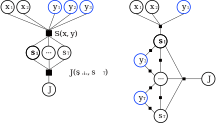
\includegraphics[width=0.8\linewidth]{images/ch7/graphs.png}
    \caption{Left: a factored graphical model in the form supported by the inference methods presented in Chapter~\ref{section:global_methods}, where all random choices (blue circles) are factored out into the exogenous inputs $y$. Right: a graphical model with a more complex structure, where random choices are not factored out and can depend on intermediate states.}
    \label{ch7:fig:graphical_models}
\end{figure}

In particular, this research will explore two distinct questions:
\begin{enumerate}
    \item Can we use probabilistic programming to perform causal analysis of autonomous systems, in particular answering root-cause failure analysis problems? E.g. if a robot fails to complete a task in a particular way, can we use probabilistic programming to infer the most likely cause or causes of the failure?
    \item Can we use probabilistic programming to define inference problems that search over the space of possible program structures? E.g. to search over the space of possible robot limb morphologies, or to search over symbolically-defined control policies? This will involve drawing on recently-developed methods for involutive and reversible-jump MCMC, which have been applied to inference problems with hierarchical models~\cite{cusumano-townerAutomatingInvolutiveMCMC2020}.
\end{enumerate}

% Explain gap between existing approach (reparameterization trick/factor out all randomness into inputs to deterministic function) and probabilistic programming.

% Explain advantages that probprog may have for a design process.

% Formulate specific research goal.

\paragraph{Lessons learned for gradient-free solution methods}

A large part of this thesis is motivated by the ability to introspect program structure (e.g. through automatic differentiation) to improve the performance of design and verification algorithms. Unfortunately, there will always be problems where it is not feasible to perform this introspection; for example, if a simulator relies on proprietary code that is only available in binary form, or if there is simply not enough engineering effort available to port an existing simulator to an AD-compatible library. To handle these cases, in the next year I will explore how to apply the lessons learned from gradient-based design and verification to accelerate gradient-free solution methods, including through the use of gradient estimation and proxy modeling.

The main output of this line of research will be a gradient-free MCMC inference algorithm that uses a combination of proxy modeling and gradient estimation to accelerate convergence to the target distribution. This algorithm will be evaluated on a range of challenging problems, including problems with stiff gradients, discontinuities, and flat regions.

%!TEX root = ./main.tex

\section{Milestones and Program Logistics}\label{section:planning}

\subsection{Classes and Degree Milestones}

Table~\ref{ch8:tab:course_requirements} shows my competed coursework, and Table~\ref{ch8:tab:degree_milestones} shows completed and anticipated degree milestones.

\begin{table}[h]
    \centering
    \caption{My completed coursework, satisfying all academic requirements for the doctoral program. Major: autonomy. Minor: controls.}
    \label{ch8:tab:course_requirements}
    \begin{tabular}{llll}
        Semester    & Class                                             & Req.       & Status    \\ \hline
        Fall 2019   & 16.413 Principles of Autonomy \& Decision Making  & major      & completed \\
        Fall 2019   & 6.255 Optimization Methods                        & major/math & completed \\
        Spring 2020 & 16.412 Cognitive Robotics                         & major      & completed \\
        Spring 2020 & 6.832 Underactuated Robotics                      & minor      & completed \\
        Fall 2020   & 18.385 Nonlinear Dynamics and Chaos               & minor/math & completed \\
        Fall 2020   & 2.160 Identification, Estimation, and Learning    & minor      & completed \\
        Spring 2021 & 16.S398 Formal Methods in Autonomy                & major      & completed \\
        Fall 2021   & 6.843: Robotic Manipulation                       & major      & completed \\
        Fall 2021   & 16.995 Doctoral Research \& Communication Seminar & RPC        & completed
    \end{tabular}
\end{table}

\begin{table}[h]
    \centering
    \caption{Milestones towards my completion of the doctoral degree. Italicized milestones are anticipated.}
    \label{ch8:tab:degree_milestones}
    \begin{tabular}{rl}
        Fall 2019 (September)       & Began studies at MIT                           \\
        Fall 2020 (December)        & Field evaluation complete                      \\
        Spring 2021 (May)           & Masters thesis submitted                       \\
        Fall 2022 (September)       & Committee meeting \#1                          \\
        Summer 2023 (June)          & Commitee meeting \#2 and thesis proposal       \\
        \textit{Fall 2023}          & \textit{Committee meeting \#3}                 \\
        \textit{Spring 2024}        & \textit{Committee meeting \#4 and green light} \\
        \textit{Spring/Summer 2024} & \textit{Thesis defense}
    \end{tabular}
\end{table}

\subsection{Research Schedule}

My thesis research will proceed in stages, as outlined below.

Spring 2022
\begin{enumerate}
    \item Certifiable robot design optimization using differentiable programming
          \begin{enumerate}
              \item Develop design optimization tool using automatic differentiation
              \item Develop statistical robustness certification tool based on extremal types theorem
              \item Hardware deployment
              \item Accepted to RSS 2022
          \end{enumerate}
    \item Robust counterexample-guided optimization with temporal logic specifications
          \begin{enumerate}
              \item Define two-player zero-sum game between the designer and the verifier
              \item Incorporate counterexamples from the verifier to guide robust design optimization
              \item Use differentiable signal temporal logic for complex task specification
              \item Submitted to IROS 2022
          \end{enumerate}
\end{enumerate}

Fall/Winter 2022
\begin{enumerate}
    \item Improving design optimization and verification through automated failure mode discovery
          \begin{enumerate}
              \item Use differentiable programming and sequential MCMC to discover a diverse set of possible failure modes.
              \item Use counterexamples from all failure modes to guide robust design optimization
          \end{enumerate}
\end{enumerate}

Spring 2023
\begin{enumerate}
    \item Extend failure mode prediction and mitigation framework to challenging new problem domains, including:
          \begin{enumerate}
              \item Perception-in-the-loop controllers, through the use of differentiable rendering,
              \item Deep neural network controllers.
          \end{enumerate}
\end{enumerate}

\textit{Fall 2023}
\begin{enumerate}
    \item Develop MCMC-based algorithm for safety verification and optimization of systems with discrete structure (e.g. involutive MCMC for robot manipulators with variaible morphologies).
    \item Write thesis
\end{enumerate}

\textit{Spring 2024}
\begin{enumerate}
    \item Write thesis
    \item Defend thesis and graduate
\end{enumerate}


%---------------------------------------------------------------------------------------------%
% Bibliography
%---------------------------------------------------------------------------------------------%
\newpage

%-----------------------%
% automatic bib entries %
%-----------------------%
% enter your bibliographies using a .bib file
% for most formats, the unsrt argument (unsorted) will list the bibliographies as cited in the 
% text, rather than sorting them alphabetically. For the \bibliography entries, much like the 
% \graphicspath entries, each relative file directory is separated by a comma, no space,
% followed by the .bib file name, without the .bib extension
\bibliographystyle{apalike}
\bibliography{main}
% example: \bibliography{../bib/bib_example,../bib/bib_example2,../bib/bib_example3}


% %---------------------------------------------------------------------------------------------%
% % Appendix
% %---------------------------------------------------------------------------------------------%
\newpage
\appendix
\section{Appendix: Details on local methods}

\subsection{AD-enabled design optimization}

To develop a general-purpose, efficient, and robust design optimization framework for autonomous systems, we must address three main challenges. First, how can we ensure that the system is \textit{flexible}, not requiring large amounts of work to specialize the framework to particular application domains. Second, how can we incorporate \textit{robustness} into the design optimization process, to minimize the sensitivity of the optimized design to variation in the exogenous parameters. Finally, how can we achieve both of these goals \textit{efficiently}, making use of gradients wherever possible to accelerate the search for high-performing designs.

\paragraph{Flexibility} Most robots are composed of many interacting subsystems, and different subsystems are typically modeled using different levels of abstraction. Although some tools may aid in designing certain subsystems (e.g. Simulink for controllers, SolidWorks for hardware), these tools cover only a small part of the overall robotics design problem, which includes sensing, actuation, perception, navigation, control, and decision-making subsystems. Since few robotic systems are exactly alike, an effective design tool must allow the user to select an appropriate level of abstraction for the problem at hand.

When it comes to managing complexity in a general-purpose design framework, programming languages are a natural tool. They allow users (i.e. programmers) to define precisely which abstractions are appropriate for any given application (e.g. by defining appropriate class hierarchies and function interfaces) without sacrificing generality. To take advantage of this expressivity, we can view engineering designs as programs that define the behavior of the system given suitable choices for design structure and parameters. We can then use automatic differentiation to derive gradients connecting these parameters to the system's behavior and optimize accordingly. This view is inspired by recent work in 3D design optimization~\cite{cascaval2021differentiable}, aircraft design~\cite{sharpe_thesis}, and machine learning~\cite{paszkePyTorchImperativeStyle2019,jax2018github}.

\paragraph{Robustness} Robots operate in dynamic environments that cannot be fully specified \textit{a priori}, and nonlinear interactions between the robot and its environment can make this uncertainty difficult to quantify. Nevertheless, we must account for this uncertainty during the design process and ensure that our designs perform robustly.

Due to this uncertainty, simply minimizing the expected value of the cost $\expectation_{y \sim \cY} \big[ J\pn{S\pn{x, y}} \big]$ can lead to myopic behavior where exceptional performance for some values of $y$ compensates for poor performance on other values; this is related to the phenomenon of ``reward hacking'' in reinforcement learning~\cite{amodei2016_ai_safety}. Ideally, we would like our designs to be robust to variations in exogenous parameters: changing $y$ should not cause the performance to change much. We can include this requirement as a heuristic by penalizing the variance of $J$. Intuitively, this heuristic ``smooths'' the cost function with respect to the exogenous parameters: regions of high variance (containing sharp local minima) are penalized, while regions of low variance are rewarded. This heuristic leads us to the \textit{variance-regularized robust design optimization problem}:
\begin{subequations}\label{app:ch5:eq:design_optimization_nlp_generic}
    \begin{align}
        \min_{x \in \cX} & \quad \expectation_{y \sim \cY} \Big[ J\circ S\pn{x, y} \Big] + \lambda \rm{Var}_{y\sim\cY}\Big[ J\circ S\pn{x, y} \Big] \label{app:ch5:eq:design_optimization_objective_generic}
    \end{align}
\end{subequations}
Practically, we replace the expectation and variance with unbiased estimates over $N$ samples $y_i \sim \cY, i=1,\ldots,N$.
\begin{subequations}\label{app:ch5:eq:design_optimization_nlp}
    \begin{align}
        \min_{x \in \cX} & \quad \frac{1}{N}\sum_{i=1}^{N} \Big[J\circ S\pn{x, y_i}\Big] + \lambda \left[ \frac{\sum_{i=1}^N \pn{J\circ S\pn{x, y_i}}^2}{N-1} - \frac{\pn{\sum_{i=1}^N J\circ S\pn{x, y_i}}^2}{(N-1)N} \right] \label{app:ch5:eq:design_optimization_objective}
    \end{align}
\end{subequations}

\paragraph{Efficiency} Of course, this Monte-Carlo estimate of the variance will require multiple evaluations of $J\circ S$ (where $\circ$ denotes function composition) to evaluate~\eqref{app:ch5:eq:design_optimization_objective}. Since $S$ might itself be expensive to evaluate, approximating the gradients of \eqref{app:ch5:eq:design_optimization_objective} using finite differences or a stochastic gradient estimate will impose a large computational cost ($2nN$ additional evaluations of $J\circ S$ and $c_i$ at each step for finite differences). Instead, we can turn to automatic differentiation (AD) to directly compute these gradients with respect to $x$, which we can use with any off-the-shelf gradient-based optimization engine. The precise choice of optimization algorithm is driven by the constraints and is not central to our framework. If $\cX$ is defined by hyper-rectangle bounds on $x$, then algorithms like L-BFGS-B may be used, but if the constraints are more complex then sequential quadratic programming or interior-point methods may be used.

In this framework, the user need only implement the simulator and cost function for their specific problem using a differentiable programming framework like the JAX library for Python~\cite{jax2018github}, and this implementation can be used automatically for efficient gradient-based optimization. By implementing a library of additional building blocks in this AD paradigm (e.g. estimation algorithms like the EKF), we can provide an AD-based design optimization tool that strikes a productive balance between flexibility and ease of use.

\subsection{Details on multi-agent manipulation case study}

Consider a case study where two mobile robots must collaborate to move a large object. In this setting, two ground robots must collaborate to push a box from its current location to a target pose (as in Fig.~\ref{ch5:fig:mam_hw}). Given the desired box pose and the current location of each robot, a neural network plans a trajectory for each robot, which the robots then track using a feedback controller ($x$ includes both the neural network parameters and the tracking controller gains, with a total of 454 design parameters). The exogenous parameters include the coefficient of friction for each contact pair, the mass of the box, the desired pose of the box, and the initial pose for each robot (a total of 13 exogenous parameters; we vary the desired box pose and initial robot poses to prevent over-fitting during optimization). The cost function is simply the squared error between the desired box pose (including position and orientation) and its true final pose after a \SI{4}{s} simulation. We implement the contact dynamics simulator, trajectory planning neural network, and path tracking controller in Python using JAX.

This case study involves interactions between planning and control subsystems, complicated dynamics, and a high-dimensional design space (>400 design parameters). This example also showcases a different interpretation of the exogenous parameters: instead of representing true sources of randomness, these parameters represent quantities that are simply unknown at design-time. For example, the target position for the box is not random in the same way as sensor noise in the previous example, but since we cannot choose this value at design-time it must be included in $y$. As a result, minimizing the expected cost with respect to variation in $y$ yields a solution that achieves good performance for many different target poses, enabling the user to select one at run-time and be confident that the design will perform well.

To solve this design problem, the neural network parameters are initialized i.i.d. according to a Gaussian distribution, and the tracking controller gains are set to nominal values. We then optimize the parameters using $N = 512$, $\lambda = 0.1$, and L-BFGS-B back-end. This optimization took 45 minutes \SI{32}{s} on a laptop computer with no GPU (\SI{8}{GB} of RAM and a \SI{1.8}{GHz} 8-core CPU). Fig.~\ref{ch5:fig:mam_hw} shows a comparison between the initial and optimized strategies, and Fig.~\ref{app:ch5:fig:mam_more} in the appendix shows additional examples of the optimized behavior. The target pose is drawn uniformly $[p_x, p_y, x] \in[0, 0.5]^2 \times [-\pi/4, \pi/4]$, and the optimized design achieves a mean squared error of $0.0964$.

We tested the optimized design in hardware, again using the Turtlebot 3 platform. An overhead camera and AprilTag~\cite{olson2011tags} markers were used to obtain the location of the box and each robot. At execution, each robot first moves to a designated starting location near the box, plans a trajectory using the neural network policy, and tracks that trajectory at \SI{100}{Hz} until the box reaches its desired location or a time limit is reached. Results from this hardware experiment are shown in Fig.~\ref{ch5:fig:mam_hw}, and a video is included in the supplementary materials. No parameter tuning or estimation was needed to transfer to hardware.

\begin{figure}[t]
    \centering
    \includegraphics[width=\linewidth]{images/ch5/mam_more.png}
    \caption{Additional examples of optimized multi-agent manipulation behavior in simulation, showing that the optimized strategy reaches the goal in most cases. Each example shows the results of executing the optimized pushing strategy for \SI{4}{s} with a randomly selected set of friction coefficients, random target pose, and random initial robot poses. Light/dark colors indicate initial/final positions, and the striped box indicates the target pose.}
    \label{app:ch5:fig:mam_more}
\end{figure}

To assess the robustness and efficiency of this design optimization method, we must answer a number of questions. For instance, how does automatic differentiation compare with other methods for estimating the gradient (e.g. finite differences)? What benefit does variance regularization in problem~\eqref{ch5:eq:design_optimization_nlp} bring? We answer these questions here using an ablation study where we attempt to isolate the impact of each of these features.

First, why use automatic differentiation? On the one hand, AD allows us to estimate the gradient with only a single evaluation of the objective function, while other methods (such as finite differences, or FD) require multiple evaluations. On the other hand, AD necessarily incurs some overhead at runtime, making each AD function call more expensive than those used in an FD scheme. Additionally, some arguments~\cite{suh2021_bundled_gradients} suggest that exact gradients may be less useful than finite-difference or stochastic approximations when the objective is stiff or discontinuous. We compare AD with a 3-point finite-difference method by re-solving problem~\eqref{ch5:eq:design_optimization_nlp} for both case studies, keeping all parameters constant ($N=512$, $\lambda=0.1$, same random seed) and substituting the gradients obtained using AD for those computed using finite differences. Fig.~\ref{ch5:fig:ablation} shows the results of this comparison. In the sensor placement example, AD achieves a lower expected cost and cost variance, and it runs in 32\% less time. In the collaborative manipulation example, both methods achieve similar expected cost and variance, but the AD version runs nearly 19x faster. These results lead us to conclude that AD enables more effective optimization than finite differences and is an appropriate choice for our framework.

The next question is whether variance regularization brings any benefit to the design optimization problem. To answer this question, we compare the results of re-solving both case studies with variance weight $\lambda = 0.1$ and $\lambda = 0$. These results are shown in Fig.~\ref{ch5:fig:ablation}; surprisingly, in the sensor placement example we see that the variance-regularized problem results in a lower expected cost, contrary to the intuition that regularization requires a trade off with increased expected cost. We expect that this lower expected cost may be a result of the regularization term smoothing the objective with respect to the exogenous parameters. However, these benefits are less pronounced than the benefits from automatic differentiation, and we see more benefit in the sensor-placement example reported in~\cite{dawsonCertifiableRobotDesign2022a} than in the multi-agent manipulation problem.

\begin{figure}[t]
    \centering
    \begin{subfigure}[t]{0.25\linewidth}
        \centering
        \includegraphics[width=\linewidth]{images/ch5/agv_ad_fd_ablation.png}
        \caption{AD vs. FD; sensor placement}
    \end{subfigure}%
    % \ \\
    % \ \\
    \begin{subfigure}[t]{0.25\linewidth}
        \centering
        \includegraphics[width=\linewidth]{images/ch5/mam_ablation_ad_fd.png}
        \caption{AD vs. FD; manipulation}
    \end{subfigure}%
    \begin{subfigure}[t]{0.25\linewidth}
        \centering
        \includegraphics[width=\linewidth]{images/ch5/agv_vr_ablation.png}
        \caption{VR; sensor placement}
    \end{subfigure}%
    % \ \\
    % \ \\
    \begin{subfigure}[t]{0.25\linewidth}
        \centering
        \includegraphics[width=\linewidth]{images/ch5/mam_ablation_vr.png}
        \caption{VR; manipulation}
    \end{subfigure}
    \caption{(a)-(b) Improvement of automatic differentiation (AD) over finite differences (FD) in both case studies. (c)-(d) Effect of variance regularization (VR) in both case studies.}
    \label{app:ch5:fig:ablation}
\end{figure}

\subsection{Details on satellite trajectory planning case study}

We can express this problem using dynaimcs in the Clohessy-Wiltshire-Hill coordinate frame~\cite{jewisonSpacecraftBenchmarkProblem2016}, which assumes that the target's orbit is circular and constructs a coordinate frame with the origin at the target, the $x$-axis pointing away from the Earth, the $y$-axis pointing along the target's orbit, and the $z$-axis pointing out of the orbital plane. In this frame, the chaser's dynamics are approximately linear, with positions $p_x$, $p_y$, $p_z$ and velocities $v_x$, $v_y$, $v_z$ varying according to controlled thrust in each direction $u_x$, $u_y$, $u_z$:
\begin{align*}
    \mat{\dot{p}_x              \\ \dot{p}_y \\ \dot{p}_z \\ \dot{v}_x \\ \dot{v}_y \\ \dot{v}_z} = \mat{
    v_x                         \\
    v_y                         \\
    v_z                         \\
    3n^2 p_x + 2n v_y + u_x / m \\
    -2n v_x + u_y / m           \\
        -n^2 p_z + u_z / m
    }
\end{align*}
%
$n = \sqrt{\mu / a^3}$ is the mean-motion of the target, determined by the Earth's gravitational constant $\mu = \SI{3.986e14}{m^3/s^2}$ and the target's altitude $a$ (i.e. the length of the semi-major orbital axis, \SI{353}{km} in low Earth orbit). $m = \SI{500}{kg}$ is the mass of the chaser satellite~\cite{jewisonSpacecraftBenchmarkProblem2016}.

%---------------------------------------------------------------------------%
%								 End Document								%
%---------------------------------------------------------------------------%
\end{document}
